\section{Algoritmos genéticos}

Algoritmos genéticos (AGs) são uma meta-heurística baseada em princípios de seleção natural para obtenção de boas soluções para problemas. As características dos AGs os tornam excelentes ferramentas para vários propósitos diferentes. Nesta seção, são descritos os passos que todos os AGs devem seguir, e são apresentadas aplicações destes algoritmos.

\subsection{Estrutura de algoritmos genéticos}

Os AGs simulam mecanismos evolutivos para obter soluções para problemas. Para tal, os AGs dependem de uma operação de conversão de soluções para cromossomos e vice-versa. Um cromossomo é uma estrutura de dados que contém as informações necessárias para reconstruir e avaliar uma solução. Geralmente, utilizam-se vetores de números para representar um cromossomo. Um exemplo simples de cromossomo é descrito por \textcite{HERMAWANTO2013}, que propõe um AG para resolução de um problema de minimização de quatro variáveis. Para resolver este problema, o autor representa os cromossomos como vetores de quatro números inteiros, cada um correspondendo ao valor de uma variável. Em problemas mais complexos, a conversão cromossomial pode ser mais complicada. No caso do exemplo citado, como os genes informam diretamente os valores das variáveis do problema, diz-se que a informação necessária para decodificar o cromossomo está no seu \emph{genótipo}. No entanto, se os valores nos genes precisarem passar por algum processo de ``tradução'' para corresponderem a informações concretas, diz-se que as informações das variáveis estão contidas no \emph{fenótipo} do cromossomo \cite{GENDREAU2010}.

Após a determinação do processo de conversão cromossomial supracitado, é necessário determinar uma função de aptidão (\emph{fitness}), ou seja, uma função que retorne valores através dos quais seja possível comparar cromossomos. Na realidade, tal função não precisa ser matematicamente objetiva -- o processo de classificação de uma solução pode ser subjetivo \cite{SASTRY2005}, o que significa que AGs podem ser utilizados para resolver problemas de otimização de caixa preta (\emph{blackbox}), ou seja, problemas cuja função objetivo ou restrições não são conhecidas ou bem-definidas \cite{ALARIE2021}. Feito isso, resta implementar os passos seguintes, cuja descrição é baseada, principalmente, na obra de \textcite{SASTRY2005}.

\subsubsection*{Inicialização}

Na etapa de inicialização, as primeiras soluções para o problema são geradas. Tais soluções podem ser completamente aleatórias ou advir de heurísticas de construção especializadas. Uma diferença importante entre os AGs e as técnicas de recozimento simulado (RS) está no fato que o RS mantém uma única solução ao longo de todo o processo de resolução do problema, ao passo que nos AGs existem $n \geq 2$ soluções. O conjunto de soluções é chamado de \emph{população}, e traz consigo a vantagem de explorar, concorrentemente, várias alternativas diferentes de resolução de problema (a este respeito, o trabalho de \textcite{MURAWSKI2016} é bastante elucidativo, mostrando como vários agentes, utilizando diferentes heurísticas, descobrem uma parte muito maior do conjunto solução de um problema do que agentes individuais).

Apesar do poder de exploração da população, é necessário escolher o seu tamanho com cautela. Populações muito pequenas podem apresentar baixa variedade cromossomial e, consequentemente, convergir para ótimos locais ao longo do processo evolutivo. Por outro lado, populações muito grandes podem ser computacionalmente ineficientes, se populações menores forem capazes de atingir os mesmos resultados \cite{ROEVA2013}. Para problemas com custo computacional muito elevado, \textcite{DELAHAYE2019} recomendam a utilização de métodos sem população, como o RS.

\subsubsection*{Avaliação}

Na avaliação, os cromossomos da população atual são avaliados pela função de aptidão. Como abordado anteriormente, esta função pode ser objetiva ou subjetiva -- o importante é que, ao fim do processo, os cromossomos possam ser comparados. Quando o valor da função de aptidão é objetivo, é necessário especificar o que faz de um valor melhor ou pior do que o outro. Por exemplo, no AG de \textcite{HERMAWANTO2013} para resolução de problemas de minimização, a função de aptidão é a própria função a minimizar e, portanto, soluções que obtiverem valores menores serão melhores. Se o problema a resolver fosse de maximização, valores maiores seriam melhores.

\subsubsection*{Seleção}

O processo de seleção leva em conta os resultados da etapa de avaliação para definir casais (pares) de cromossomos. Os métodos de seleção costumam implementar processos estocásticos em que os cromossomos com avaliações melhores são favorecidos. Na sequência, são abordados alguns métodos.

\textbf{Método da roleta:} Sejam $n \geq 2$ o tamanho da população e $q_i$ ($i = 1, \dots, n$) os valores de aptidão de cada solução. A cada solução $i$ é associada uma probabilidade $p_i = q_i / \sum_{j=1}^{n}q_j$ de que $i$ seja selecionada. À solução 1 fica atribuído o intervalo $I_1 = [0, p_1]$. A partir disso, é possível determinar os intervalos das soluções $k = 2, \dots, n$, em sequência, com $I_k = \left(\sum_{j=1}^{k-1}p_j, \sum_{j=1}^{k}p_j\right]$. Evidentemente, $\cup_{j=1}^{n}I_j = [0, 1]$, então, gera-se um valor aleatório $r \in [0, 1]$, de modo que $r \in I_k$ significa que a solução $k$ deve ser selecionada \cite{CARVALHO,SASTRY2005}.

A título de exemplo, supõe-se uma população de cinco soluções, cujos dados são apresentados na \cref{tab:roleta}.

\begin{table}[ht]
    \centering
    \caption{}
    \label{tab:roleta}
    \begin{tabular}{cccc}
        \toprule
        Solução ($k$) & Aptidão ($q_k$) & Probabilidade ($p_k$) & Intervalo ($I_k$)\\
        \midrule
        1 & 4.52 & 0.156 & [0, 0.156]\\
        2 & 9.04 & 0.313 & (0.156, 0.469]\\
        3 & 7.33 & 0.254 & (0.469, 0.723]\\
        4 & 3.21 & 0.111 & (0.723, 0.834]\\
        5 & 4.79 & 0.166 & (0.834, 1]\\
        \bottomrule 
    \end{tabular}
\end{table}

\textbf{Método de \emph{ranking}:} Neste método, ordenam-se as soluções da pior para a melhor, baseado em seus valores de aptidão. Em seguida, a cada solução $k$ é atribuido um valor $r_k$ equivalente à posição da solução na lista ordenada. Desta forma, a pior solução tem $r_k = 1$, e a melhor solução tem $r_k = n$. Estes valores substituem os valores de aptidão durante o processo de seleção, e o método procede como o da roleta.

Aplicando-se o método de \emph{ranking} às soluções da \cref{tab:roleta}, obtém-se um resultado diferente do método da roleta. A \cref{fig:roleta e ranking} compara visualmente as probabilidades geradas por ambos os métodos. Como as probabilidades no método de \emph{ranking} são independentes dos valores de aptidão das soluções, este método pode ser mais interessante quando poucas soluções têm valor de aptidão muito mais alto do que as demais, pois aumenta as chances de soluções de menos qualidade serem selecionadas \cite{YADAV2017}. Apesar de isso parecer contraintuitivo, é importante permitir que soluções piores contribuam para o desenvolvimento genético da população, pois isso permite uma maior exploração do conjunto de soluções.

\begin{figure}[ht]
    \centering
    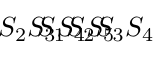
\begin{tikzpicture}
        \matrix[column sep = 1cm]{
        \pie{15.6/$S_1$, 31.3/$S_2$, 25.4/$S_3$, 11.1/$S_4$, 16.6/$S_5$}
        &
        \pie{13.3/$S_1$, 33.3/$S_2$, 26.7/$S_3$, 20/$S_4$, 6.7/$S_5$}\\
        };
    \end{tikzpicture}
    \caption{Probabilidades de seleção de soluções pelos métodos da roleta (esquerda) e de \emph{ranking} (direita).}
    \label{fig:roleta e ranking}
\end{figure}

\textbf{Método de torneio:} Seja $P$ a população de soluções de um problema. O método de torneio escolhe subconjuntos $S_i \subseteq P$  de soluções da população e então seleciona a melhor solução de cada subconjunto $S_i$. Assim como o método de \emph{ranking}, este método pode aumentar as probabilidades de seleções piores serem selecionadas, dependendo da maneira como os subconjuntos $S_i$ forem determinados. Geralmente, este método é implementado com torneios de duas soluções, o que o torna uma forma muito rápida de seleção e garante maior variedade de qualidade das soluções escolhidas \cite{SHUKLA2015}.

\textbf{Método de Boltzmann:} Este método é similar ao RS. Existe um parâmetro de temperatura que diminui ao longo do tempo. A altas temperaturas, as chances de selecionar quaisquer soluções são quase iguais. Já a temperaturas mais baixas, as chances de selecionar soluções melhores aumentam.